\documentclass[handout]{beamer}

\usepackage{graphicx}
\usepackage{tikz-cd}

\title{EPIT Lecture 5.2\\ The Universal Cover of the Circle}
\author{Egbert Rijke}
\date{Friday, April 16th 2020}

\setbeamertemplate{caption}{\raggedright\insertcaption\par}

\mathchardef\usc="2D
\newcommand{\N}{\mathbb{N}}
\newcommand{\Z}{\mathbb{Z}}
\newcommand{\UU}{\mathcal{U}}
\newcommand{\brck}[1]{\|#1\|}
\newcommand{\Brck}[1]{\left\|#1\right\|}
\newcommand{\trunc}[2]{\|#2\|_{#1}}
\newcommand{\Trunc}[2]{\left\|#2\right\|_{#1}}
\newcommand{\unit}{\mathbf{1}}
\newcommand{\sphere}[1]{S^{#1}}
\newcommand{\isnull}{\mathsf{is\usc{}null}}
\newcommand{\htpy}{\sim}
\newcommand{\apbinary}{\mathsf{ap\usc{}bin}}
\newcommand{\Glob}{\mathsf{Glob}}
\newcommand{\typeGlob}{\mathsf{type}}
\newcommand{\relGlob}{\mathsf{rel}}
\newcommand{\homGlob}{\mathsf{hom}}
\newcommand{\maphomGlob}{\mathsf{map}}
\newcommand{\cgrhomGlob}{\mathsf{cgr}}
\newcommand{\bihomGlob}{\mathsf{bihom}}
\newcommand{\mapbihomGlob}{\mathsf{map}}
\newcommand{\cgrbihomGlob}{\mathsf{cgr}}
\newcommand{\ct}{\bullet}
\newcommand{\isconstant}[2]{\mathsf{is\usc{}}(#1,#2)\mathsf{\usc{}constant}}
\newcommand{\ap}{\mathsf{ap}}
\newcommand{\interchange}{\mathsf{interchange}}
\newcommand{\refl}{\mathsf{refl}}
\newcommand{\eh}{\mathsf{eckmann\usc{}hilton}}
\newcommand{\blank}{\mathord{\hspace{1pt}\text{--}\hspace{1pt}}}
\newcommand{\EM}{\mathsf{EM}}
\newcommand{\baseS}{\mathsf{base}}
\newcommand{\loopS}{\mathsf{loop}}
\newcommand{\apd}{\mathsf{apd}}
\newcommand{\tr}{\mathsf{tr}}
\newcommand{\idfunc}{\mathsf{id}}
\newcommand{\mulcircle}{\mu}
\newcommand{\basemulcircle}{\mathsf{base\usc{}mul}_{\sphere{1}}}
\newcommand{\loopmulcircle}{\mathsf{loop\usc{}mul}_{\sphere{1}}}
\newcommand{\htpyidcircle}{H}
\newcommand{\basehtpyidcircle}{\alpha}
\newcommand{\loophtpyidcircle}{\beta}
\newcommand{\invcircle}{\mathsf{inv}_{\sphere{1}}}
\newcommand{\evbase}{\mathsf{ev\usc{}base}}
\newcommand{\eqhtpy}{\mathsf{eq\usc{}htpy}}
\newcommand{\apply}[2]{#1(#2)}
\newcommand{\equiveq}{\mathsf{equiv\usc{}eq}}
\newcommand{\succZ}{\mathsf{succ}}
\newcommand{\bool}{\mathsf{bool}}

\setbeamertemplate{navigation symbols}{}
\setbeamertemplate{footline}[frame number]{}

\begin{document}

\begin{frame}
  \maketitle
\end{frame}

\begin{frame}
  \frametitle{Main theorem of this lecture}
  \begin{definition}
    Let $A$ be a type equipped with a point $a:A$. Then we define the \textbf{loop space} of $A$ at $a$ to be the type
    \begin{equation*}
      \Omega(A,a):= (a=a).
    \end{equation*}
    It comes equipped with the point $\refl:\Omega(A,a)$.
  \end{definition}

  \begin{theorem}
    There is an equivalence
    \begin{equation*}
      \Omega(\sphere{1},\baseS)\simeq \Z.
    \end{equation*}
  \end{theorem}
\end{frame}

\begin{frame}
  \begin{theorem}[The fundamental theorem of identity types]
    Consider a type $A$ with base point $a:A$. Let $B$ be a type family over $A$ equipped with a point $b:B(a)$. Then the following are equivalent:
    \begin{enumerate}
    \item The family of maps
      \begin{equation*}
        f : (a=x)\to B(x)
      \end{equation*}
      indexed by $x:A$, given by $f(\refl):=b$, is a family of equivalences.
    \item The type
      \begin{equation*}
        \sum_{(x:A)}B(x)
      \end{equation*}
      is contractible.
    \end{enumerate}
  \end{theorem}
\end{frame}

\begin{frame}
  \frametitle{The encode-decode method}
  Suppose we want to show that $\Omega(A,a)\simeq G$, for some type $G$.
  \begin{itemize}
  \item First define a type family
    \begin{equation*}
      B : A \to \UU
    \end{equation*}
    equipped with an equivalence $e:B(a)\simeq G$. $B$ is said to \textbf{encode} the identity type of $A$.
  \item Then show that the total space
    \begin{equation*}
      \sum_{(x:A)}B(x)
    \end{equation*}
    is contractible.
  \end{itemize}
  By the fundamental theorem it then follows that the family of maps
  \begin{equation*}
    (a=x)\to B(x)
  \end{equation*}
  indexed by $x:A$, given by $f(\refl):=e^{-1}(1)$, is a family of equivalences. In particular, we obtain
  \begin{equation*}
    (a=a)\simeq B(a)\simeq G.
  \end{equation*}
\end{frame}

\begin{frame}
  \frametitle{Encoding the identity type of $\sphere{1}$}
  Our goal is to show that $\Omega(\sphere{1},\baseS)\simeq \Z$. For the second step in the encode decode method, we have to construct a type family
  \begin{equation*}
    B : \sphere{1}\to \UU.
  \end{equation*}
  Such a family is constructed by the universal property of $\sphere{1}$(!!)
  \begin{theorem}
    The map
    \begin{equation*}
      (\sphere{1}\to\UU)\to\sum_{(X:\UU)}X\simeq X
    \end{equation*}
    given by $P\mapsto (P(\baseS),\tr_P(\loopS))$ is an equivalence. 
  \end{theorem}
\end{frame}

\begin{frame}
  \begin{proof}
    We have a commuting triangle
    \begin{equation*}
      \begin{tikzcd}[ampersand replacement=\&]
        \& (\sphere{1}\to\UU) \arrow[dl,swap,"{P\mapsto(P(\baseS),\ap_P(\loopS))}"] \arrow[dr,"{P\mapsto(P(\baseS),\tr_P(\loopS))}"] \\
        \sum_{(X:\UU)}X=X \arrow[rr,swap,"{(X,p)\mapsto(X,\equiveq(p))}"] \& \& \sum_{(X:\UU)}X\simeq X
      \end{tikzcd}
    \end{equation*}
    This triangle commutes, because
    \begin{equation*}
      \equiveq(\ap_P(q))=\tr_P(q)
    \end{equation*}
    for any identification $q:x=y$ in $\sphere{1}$.
    \begin{itemize}
    \item The bottom map is an equivalence by univalence.
    \item The left map is an equivalence by the universal property of $\sphere{1}$.
    \item Hence the right map is an equivalence.\qedhere
    \end{itemize}
  \end{proof}
\end{frame}

\begin{frame}
  \frametitle{Here's how to define a type family over $\sphere{1}$}
  Suppose we have
  \begin{align*}
    X & : \UU \\
    e & : X \simeq X.
  \end{align*}
  By the equivalence $(\sphere{1}\to\UU)\simeq\sum_{(X:\UU)}X\simeq X$ we then obtain a unique family $P:\sphere{1}\to\UU$ equipped with
  \begin{itemize}
  \item an equivalence $\alpha:X\simeq P(\baseS)$.
  \item a homotopy witnessing that the square
    \begin{equation*}
      \begin{tikzcd}[ampersand replacement=\&]
        X \arrow[d,swap,"e"] \arrow[r,"\alpha"] \& P(\baseS) \arrow[d,"\tr_P(\loopS)"] \\
        X \arrow[r,swap,"\alpha"] \& P(\baseS)
      \end{tikzcd}
    \end{equation*}
    commutes.
  \end{itemize}
\end{frame}

\begin{frame}
  \frametitle{The universal cover of $\sphere{1}$}
  
  \begin{definition}
    The \textbf{universal cover} of $\sphere{1}$ is the unique family $E$ over $\sphere{1}$ equipped with
    \begin{itemize}
    \item An equivalence $e:\Z\simeq E(\baseS)$.
    \item A homotopy $H$ witnessing that the square
      \begin{equation*}
        \begin{tikzcd}[ampersand replacement=\&]
          \Z \arrow[d,swap,"\succZ"] \arrow[r,"e"] \& E(\baseS) \arrow[d,"\tr_E(\loopS)"] \\
          \Z \arrow[r,swap,"e"] \& E(\baseS)
        \end{tikzcd}
      \end{equation*}
      commutes. Given $k:\Z$, we will write $k_E:=e(k)$. 
    \end{itemize}
  \end{definition}
\end{frame}

\begin{frame}
  \frametitle{The geometry of the universal cover of $\sphere{1}$}
  \begin{center}
    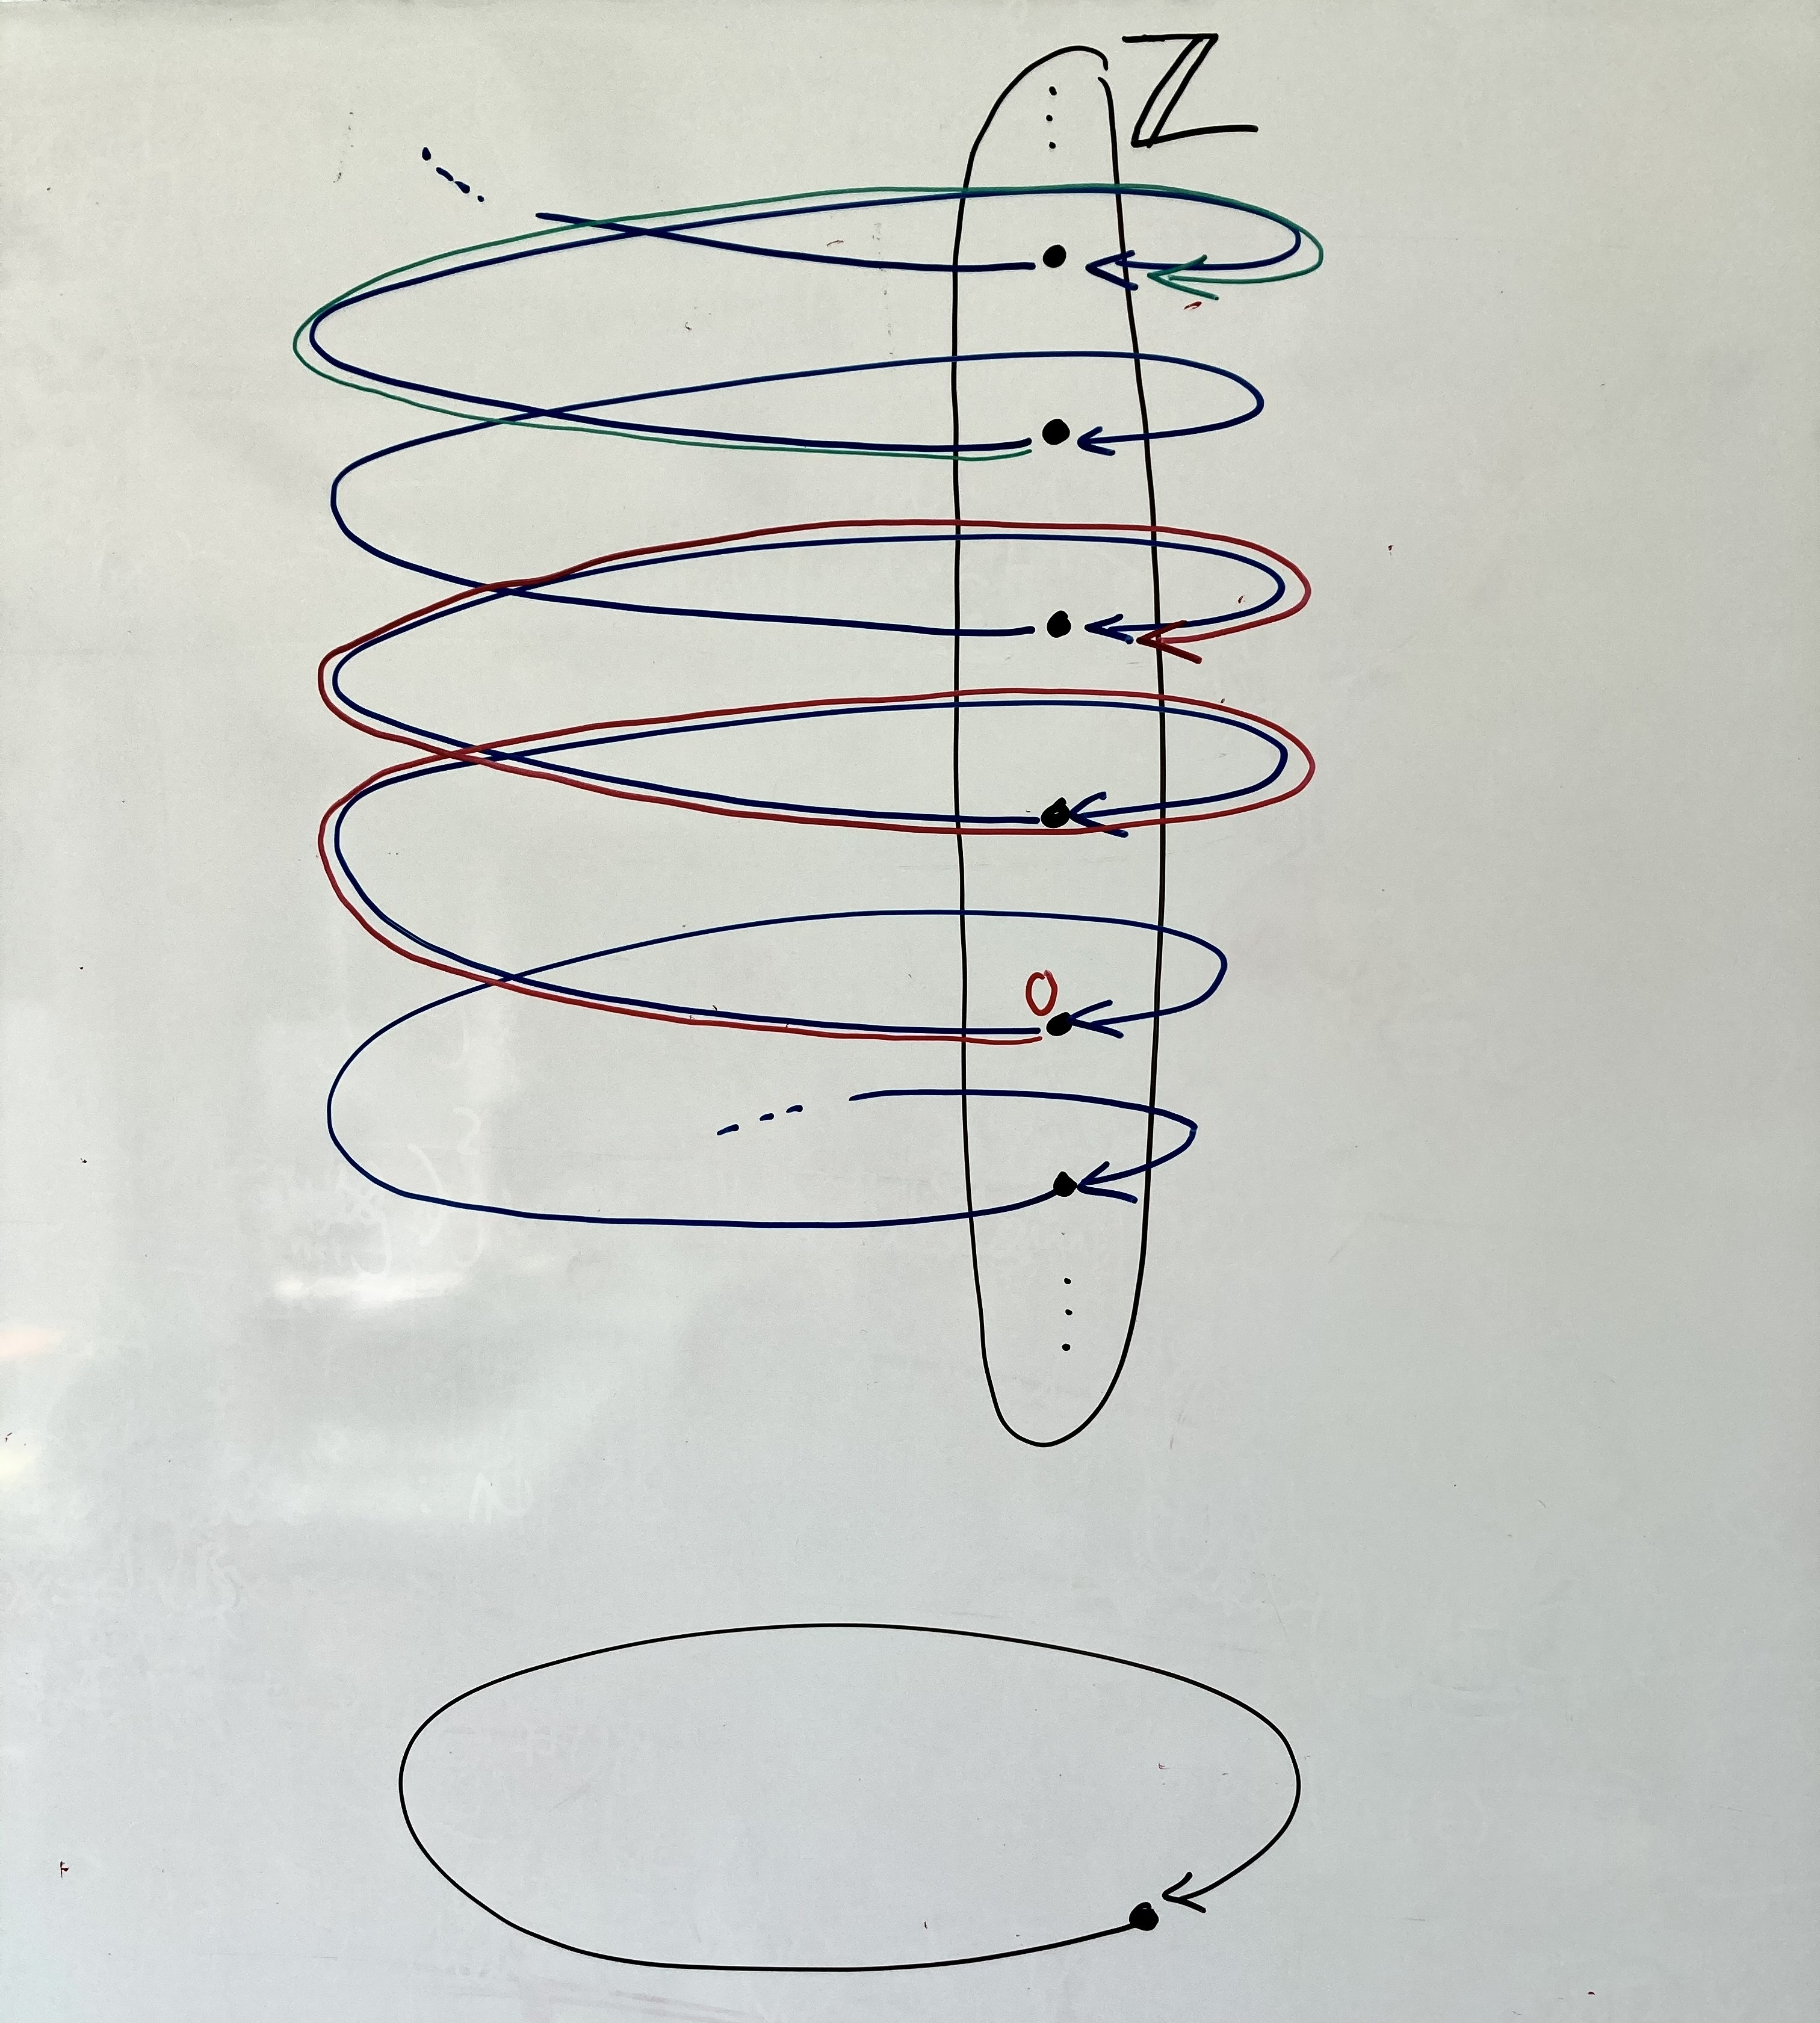
\includegraphics[width=.7\textwidth]{universal-cover-circle}
  \end{center}
\end{frame}

\begin{frame}
  \begin{lemma}[Helix]
    \begin{itemize}
    \item For any $k:\Z$ we have $\sigma_k:(\baseS,k_E)=(\baseS,\succZ(k)_E)$.
    \item For any $k:\Z$ we have $\tau_k:(\baseS,0_E)=(\baseS,k_E)$, such that 
      \begin{equation*}
        \tau_{k+1}=\tau_k\bullet \sigma_k
      \end{equation*}
      holds for any $k:\Z$.
    \end{itemize}
  \end{lemma}

  \begin{proof}
    By the characterisation of the identity types of $\Sigma$-types, we have
    \begin{equation*}
      ((\baseS,k_E)=(\baseS,\succZ(k)_E)) \simeq \sum\nolimits_{(p:\baseS=\baseS)}\tr_E(p,k_E)=\succZ(k)_E.
    \end{equation*}
    In the right hand side we have $(\loopS,H(k))$, where $H$ is the homotopy in the definition of $E$. This proves the first claim.\\[1em]

    The second claim follows by the dependent elimination principle of $\Z$.
  \end{proof}
\end{frame}

\begin{frame}
  \frametitle{The dependent elimination principle of $\Z$}
  \begin{theorem}
    Let $P:\Z\to\UU$ be a type family. If $P$ comes equipped with
    \begin{itemize}
    \item a point $p_0:P(0)$.
    \item a family of equivalences $e_k:P(k)\simeq P(\succZ(k))$ indexed by $k:\Z$.
    \end{itemize}\pause
    Then there is a dependent function $f:\prod_{(k:\Z)}P(k)$ equipped with
    \begin{itemize}
    \item an identification $f(0)=p_0$.
    \item a family of identifications
      \begin{equation*}
        f(\succZ(k))=e_k(f(k))
      \end{equation*}
      indexed by $k:\Z$.
    \end{itemize}
  \end{theorem}
\end{frame}

\begin{frame}
  \frametitle{The second step in the encode-decode method}
  \begin{theorem}
    The total space
    \begin{equation*}
      \sum_{(t:\sphere{1})}E(t)
    \end{equation*}
    is contractible, with center of contraction $(\baseS,0_E)$.
  \end{theorem}

  \begin{proof}
    Our goal is to construct the contraction, i.e.,
    \begin{equation*}
      \prod_{(x:\sphere{1})}\prod_{(u:E(x))}(\baseS,0_E)=(x,u).
    \end{equation*}
    We do this with the induction principle of $\sphere{1}$, using the family $C$ given by
    \begin{equation*}
      C(x):=\prod_{(u:E(x))}(\baseS,0_E)=(x,u)
    \end{equation*}
    \\[10cm]
    Hiding the QED symbol
  \end{proof}
\end{frame}

\begin{frame}
  \frametitle{Proof (cont.)}
  We have to define
  \begin{align*}
    p & : C(\baseS) \\
    q & : \tr_C(\loopS,p)=p.
  \end{align*}
  Note that we have a commuting square
  \begin{equation*}
    \begin{tikzcd}[ampersand replacement=\&]
      \prod_{(k:\Z)}(\baseS,0_E)=(\baseS,k_E) \arrow[r,"\alpha","\sim"'] \arrow[d,swap,"{p\mapsto \lambda k.\,p_{k+1}\bullet\sigma_k^{-1}}"] \& C(\baseS) \arrow[d,"\tr_C(\loopS)"] \\
      \prod_{(k:\Z)}(\baseS,0_E)=(\baseS,k_E) \arrow[r,swap,"\alpha","\sim"'] \& C(\baseS)
    \end{tikzcd}
  \end{equation*}
  By this square we obtain for $p:\prod_{(k:\Z)}(\baseS,0_E)=(\baseS,k_E)$, a map
  \begin{equation*}
    \Big(\prod_{(k:\Z)}p_{k+1}=p_k\bullet \sigma_k^{-1}\Big)\to \Big(\tr_C(\loopS,\alpha(p))=\alpha(p)\Big)
  \end{equation*}
  We apply the Helix lemma to finish the proof.\hfill $\square$
\end{frame}

\begin{frame}
  We have now proven our theorem:
  \begin{theorem}
    There is an equivalence
    \begin{equation*}
      \Omega(\sphere{1},\baseS)\simeq \Z.
    \end{equation*}
  \end{theorem}

  \begin{corollary}
    The circle is a $1$-type, and it is not a set. In particular, it is not contractible.
  \end{corollary}
\end{frame}

\begin{frame}
  \frametitle{Exercises}
  The \textbf{(twisted) double cover} of the circle is defined as the unique type family $D$ over $\sphere{1}$ equipped with
  \begin{itemize}
  \item An equivalence $\bool\simeq D(\baseS)$.
  \item A homotopy witnessing that the square
    \begin{equation*}
      \begin{tikzcd}[ampersand replacement=\&,row sep=1.4em]
        \bool \arrow[r,"e"] \arrow[d,swap,"\mathsf{neg}"] \& D(\baseS) \arrow[d,"\tr_{D}(\loopS)"] \\
        \bool \arrow[r,swap,"e"] \& D(\baseS)
      \end{tikzcd}
    \end{equation*}
    commutes.
  \end{itemize}
  Construct an equivalence $\alpha:{\sphere{1}}\simeq{\sum_{(t:\sphere{1})}D(t)}$ for which the triangle
  \begin{equation*}
    \begin{tikzcd}[column sep=0em,ampersand replacement=\&,row sep=small]
      \sphere{1} \arrow[rr,"\alpha"] \arrow[dr,swap,"\mathsf{deg}(2)"] \& \& \sum_{(t:\sphere{1})}D(t) \arrow[dl,"\pi_1"] \\
      \phantom{\sum_{(t:\sphere{1})}D(t)} \& \sphere{1}
    \end{tikzcd}
  \end{equation*}
  commutes, where $\mathsf{deg}(2):\sphere{1}\to\sphere{1}$ is the degree $2$ map.
\end{frame}

\end{document}
